% Graphic for TeX using PGF
% Title: /home/satenske/cours/OMGL/prl3/TD3/Diagram1.dia
% Creator: Dia v0.97.1
% CreationDate: Mon Oct  3 21:47:58 2011
% For: satenske
% \usepackage{tikz}
% The following commands are not supported in PSTricks at present
% We define them conditionally, so when they are implemented,
% this pgf file will use them.
\ifx\du\undefined
  \newlength{\du}
\fi
\setlength{\du}{15\unitlength}
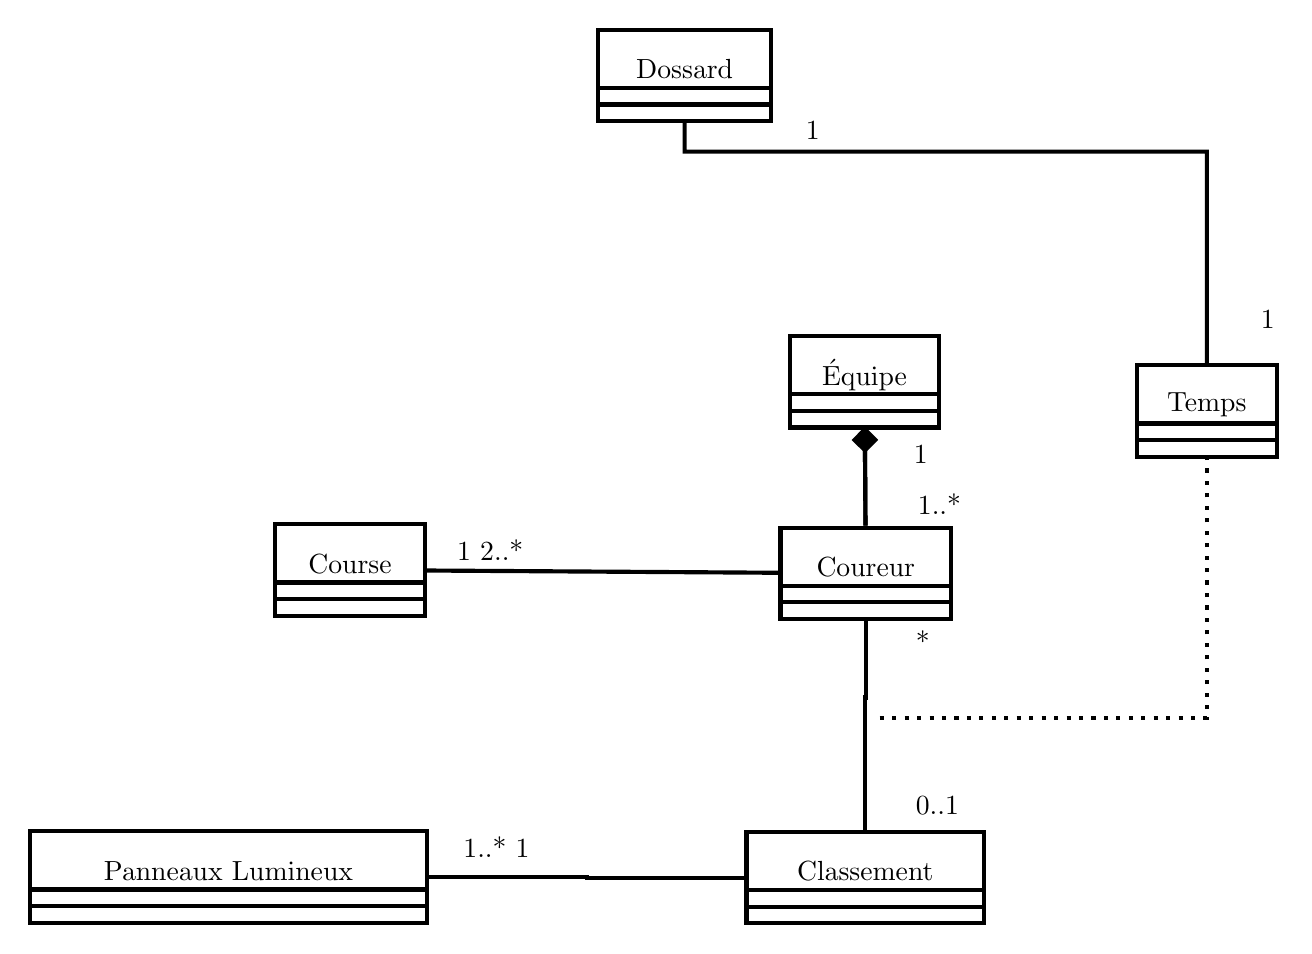
\begin{tikzpicture}
\pgftransformxscale{1.000000}
\pgftransformyscale{-1.000000}
\definecolor{dialinecolor}{rgb}{0.000000, 0.000000, 0.000000}
\pgfsetstrokecolor{dialinecolor}
\definecolor{dialinecolor}{rgb}{1.000000, 1.000000, 1.000000}
\pgfsetfillcolor{dialinecolor}
\pgfsetlinewidth{0.100000\du}
\pgfsetdash{}{0pt}
\definecolor{dialinecolor}{rgb}{1.000000, 1.000000, 1.000000}
\pgfsetfillcolor{dialinecolor}
\fill (40.150000\du,7.950000\du)--(40.150000\du,9.350000\du)--(43.512500\du,9.350000\du)--(43.512500\du,7.950000\du)--cycle;
\definecolor{dialinecolor}{rgb}{0.000000, 0.000000, 0.000000}
\pgfsetstrokecolor{dialinecolor}
\draw (40.150000\du,7.950000\du)--(40.150000\du,9.350000\du)--(43.512500\du,9.350000\du)--(43.512500\du,7.950000\du)--cycle;
% setfont left to latex
\definecolor{dialinecolor}{rgb}{0.000000, 0.000000, 0.000000}
\pgfsetstrokecolor{dialinecolor}
\node at (41.831250\du,8.900000\du){Temps};
\definecolor{dialinecolor}{rgb}{1.000000, 1.000000, 1.000000}
\pgfsetfillcolor{dialinecolor}
\fill (40.150000\du,9.350000\du)--(40.150000\du,9.750000\du)--(43.512500\du,9.750000\du)--(43.512500\du,9.350000\du)--cycle;
\definecolor{dialinecolor}{rgb}{0.000000, 0.000000, 0.000000}
\pgfsetstrokecolor{dialinecolor}
\draw (40.150000\du,9.350000\du)--(40.150000\du,9.750000\du)--(43.512500\du,9.750000\du)--(43.512500\du,9.350000\du)--cycle;
\definecolor{dialinecolor}{rgb}{1.000000, 1.000000, 1.000000}
\pgfsetfillcolor{dialinecolor}
\fill (40.150000\du,9.750000\du)--(40.150000\du,10.150000\du)--(43.512500\du,10.150000\du)--(43.512500\du,9.750000\du)--cycle;
\definecolor{dialinecolor}{rgb}{0.000000, 0.000000, 0.000000}
\pgfsetstrokecolor{dialinecolor}
\draw (40.150000\du,9.750000\du)--(40.150000\du,10.150000\du)--(43.512500\du,10.150000\du)--(43.512500\du,9.750000\du)--cycle;
\pgfsetlinewidth{0.100000\du}
\pgfsetdash{}{0pt}
\definecolor{dialinecolor}{rgb}{1.000000, 1.000000, 1.000000}
\pgfsetfillcolor{dialinecolor}
\fill (27.165000\du,-0.135000\du)--(27.165000\du,1.265000\du)--(31.337500\du,1.265000\du)--(31.337500\du,-0.135000\du)--cycle;
\definecolor{dialinecolor}{rgb}{0.000000, 0.000000, 0.000000}
\pgfsetstrokecolor{dialinecolor}
\draw (27.165000\du,-0.135000\du)--(27.165000\du,1.265000\du)--(31.337500\du,1.265000\du)--(31.337500\du,-0.135000\du)--cycle;
% setfont left to latex
\definecolor{dialinecolor}{rgb}{0.000000, 0.000000, 0.000000}
\pgfsetstrokecolor{dialinecolor}
\node at (29.251250\du,0.815000\du){Dossard};
\definecolor{dialinecolor}{rgb}{1.000000, 1.000000, 1.000000}
\pgfsetfillcolor{dialinecolor}
\fill (27.165000\du,1.265000\du)--(27.165000\du,1.665000\du)--(31.337500\du,1.665000\du)--(31.337500\du,1.265000\du)--cycle;
\definecolor{dialinecolor}{rgb}{0.000000, 0.000000, 0.000000}
\pgfsetstrokecolor{dialinecolor}
\draw (27.165000\du,1.265000\du)--(27.165000\du,1.665000\du)--(31.337500\du,1.665000\du)--(31.337500\du,1.265000\du)--cycle;
\definecolor{dialinecolor}{rgb}{1.000000, 1.000000, 1.000000}
\pgfsetfillcolor{dialinecolor}
\fill (27.165000\du,1.665000\du)--(27.165000\du,2.065000\du)--(31.337500\du,2.065000\du)--(31.337500\du,1.665000\du)--cycle;
\definecolor{dialinecolor}{rgb}{0.000000, 0.000000, 0.000000}
\pgfsetstrokecolor{dialinecolor}
\draw (27.165000\du,1.665000\du)--(27.165000\du,2.065000\du)--(31.337500\du,2.065000\du)--(31.337500\du,1.665000\du)--cycle;
\pgfsetlinewidth{0.100000\du}
\pgfsetdash{}{0pt}
\definecolor{dialinecolor}{rgb}{1.000000, 1.000000, 1.000000}
\pgfsetfillcolor{dialinecolor}
\fill (19.380000\du,11.780000\du)--(19.380000\du,13.180000\du)--(23.000000\du,13.180000\du)--(23.000000\du,11.780000\du)--cycle;
\definecolor{dialinecolor}{rgb}{0.000000, 0.000000, 0.000000}
\pgfsetstrokecolor{dialinecolor}
\draw (19.380000\du,11.780000\du)--(19.380000\du,13.180000\du)--(23.000000\du,13.180000\du)--(23.000000\du,11.780000\du)--cycle;
% setfont left to latex
\definecolor{dialinecolor}{rgb}{0.000000, 0.000000, 0.000000}
\pgfsetstrokecolor{dialinecolor}
\node at (21.190000\du,12.730000\du){Course};
\definecolor{dialinecolor}{rgb}{1.000000, 1.000000, 1.000000}
\pgfsetfillcolor{dialinecolor}
\fill (19.380000\du,13.180000\du)--(19.380000\du,13.580000\du)--(23.000000\du,13.580000\du)--(23.000000\du,13.180000\du)--cycle;
\definecolor{dialinecolor}{rgb}{0.000000, 0.000000, 0.000000}
\pgfsetstrokecolor{dialinecolor}
\draw (19.380000\du,13.180000\du)--(19.380000\du,13.580000\du)--(23.000000\du,13.580000\du)--(23.000000\du,13.180000\du)--cycle;
\definecolor{dialinecolor}{rgb}{1.000000, 1.000000, 1.000000}
\pgfsetfillcolor{dialinecolor}
\fill (19.380000\du,13.580000\du)--(19.380000\du,13.980000\du)--(23.000000\du,13.980000\du)--(23.000000\du,13.580000\du)--cycle;
\definecolor{dialinecolor}{rgb}{0.000000, 0.000000, 0.000000}
\pgfsetstrokecolor{dialinecolor}
\draw (19.380000\du,13.580000\du)--(19.380000\du,13.980000\du)--(23.000000\du,13.980000\du)--(23.000000\du,13.580000\du)--cycle;
\pgfsetlinewidth{0.100000\du}
\pgfsetdash{}{0pt}
\definecolor{dialinecolor}{rgb}{1.000000, 1.000000, 1.000000}
\pgfsetfillcolor{dialinecolor}
\fill (31.795000\du,7.245000\du)--(31.795000\du,8.645000\du)--(35.375000\du,8.645000\du)--(35.375000\du,7.245000\du)--cycle;
\definecolor{dialinecolor}{rgb}{0.000000, 0.000000, 0.000000}
\pgfsetstrokecolor{dialinecolor}
\draw (31.795000\du,7.245000\du)--(31.795000\du,8.645000\du)--(35.375000\du,8.645000\du)--(35.375000\du,7.245000\du)--cycle;
% setfont left to latex
\definecolor{dialinecolor}{rgb}{0.000000, 0.000000, 0.000000}
\pgfsetstrokecolor{dialinecolor}
\node at (33.585000\du,8.195000\du){Équipe};
\definecolor{dialinecolor}{rgb}{1.000000, 1.000000, 1.000000}
\pgfsetfillcolor{dialinecolor}
\fill (31.795000\du,8.645000\du)--(31.795000\du,9.045000\du)--(35.375000\du,9.045000\du)--(35.375000\du,8.645000\du)--cycle;
\definecolor{dialinecolor}{rgb}{0.000000, 0.000000, 0.000000}
\pgfsetstrokecolor{dialinecolor}
\draw (31.795000\du,8.645000\du)--(31.795000\du,9.045000\du)--(35.375000\du,9.045000\du)--(35.375000\du,8.645000\du)--cycle;
\definecolor{dialinecolor}{rgb}{1.000000, 1.000000, 1.000000}
\pgfsetfillcolor{dialinecolor}
\fill (31.795000\du,9.045000\du)--(31.795000\du,9.445000\du)--(35.375000\du,9.445000\du)--(35.375000\du,9.045000\du)--cycle;
\definecolor{dialinecolor}{rgb}{0.000000, 0.000000, 0.000000}
\pgfsetstrokecolor{dialinecolor}
\draw (31.795000\du,9.045000\du)--(31.795000\du,9.445000\du)--(35.375000\du,9.445000\du)--(35.375000\du,9.045000\du)--cycle;
\pgfsetlinewidth{0.100000\du}
\pgfsetdash{}{0pt}
\definecolor{dialinecolor}{rgb}{1.000000, 1.000000, 1.000000}
\pgfsetfillcolor{dialinecolor}
\fill (31.560000\du,11.860000\du)--(31.560000\du,13.260000\du)--(35.670000\du,13.260000\du)--(35.670000\du,11.860000\du)--cycle;
\definecolor{dialinecolor}{rgb}{0.000000, 0.000000, 0.000000}
\pgfsetstrokecolor{dialinecolor}
\draw (31.560000\du,11.860000\du)--(31.560000\du,13.260000\du)--(35.670000\du,13.260000\du)--(35.670000\du,11.860000\du)--cycle;
% setfont left to latex
\definecolor{dialinecolor}{rgb}{0.000000, 0.000000, 0.000000}
\pgfsetstrokecolor{dialinecolor}
\node at (33.615000\du,12.810000\du){Coureur};
\definecolor{dialinecolor}{rgb}{1.000000, 1.000000, 1.000000}
\pgfsetfillcolor{dialinecolor}
\fill (31.560000\du,13.260000\du)--(31.560000\du,13.660000\du)--(35.670000\du,13.660000\du)--(35.670000\du,13.260000\du)--cycle;
\definecolor{dialinecolor}{rgb}{0.000000, 0.000000, 0.000000}
\pgfsetstrokecolor{dialinecolor}
\draw (31.560000\du,13.260000\du)--(31.560000\du,13.660000\du)--(35.670000\du,13.660000\du)--(35.670000\du,13.260000\du)--cycle;
\definecolor{dialinecolor}{rgb}{1.000000, 1.000000, 1.000000}
\pgfsetfillcolor{dialinecolor}
\fill (31.560000\du,13.660000\du)--(31.560000\du,14.060000\du)--(35.670000\du,14.060000\du)--(35.670000\du,13.660000\du)--cycle;
\definecolor{dialinecolor}{rgb}{0.000000, 0.000000, 0.000000}
\pgfsetstrokecolor{dialinecolor}
\draw (31.560000\du,13.660000\du)--(31.560000\du,14.060000\du)--(35.670000\du,14.060000\du)--(35.670000\du,13.660000\du)--cycle;
\pgfsetlinewidth{0.100000\du}
\pgfsetdash{}{0pt}
\definecolor{dialinecolor}{rgb}{1.000000, 1.000000, 1.000000}
\pgfsetfillcolor{dialinecolor}
\fill (13.475000\du,19.175000\du)--(13.475000\du,20.575000\du)--(23.050000\du,20.575000\du)--(23.050000\du,19.175000\du)--cycle;
\definecolor{dialinecolor}{rgb}{0.000000, 0.000000, 0.000000}
\pgfsetstrokecolor{dialinecolor}
\draw (13.475000\du,19.175000\du)--(13.475000\du,20.575000\du)--(23.050000\du,20.575000\du)--(23.050000\du,19.175000\du)--cycle;
% setfont left to latex
\definecolor{dialinecolor}{rgb}{0.000000, 0.000000, 0.000000}
\pgfsetstrokecolor{dialinecolor}
\node at (18.262500\du,20.125000\du){Panneaux Lumineux};
\definecolor{dialinecolor}{rgb}{1.000000, 1.000000, 1.000000}
\pgfsetfillcolor{dialinecolor}
\fill (13.475000\du,20.575000\du)--(13.475000\du,20.975000\du)--(23.050000\du,20.975000\du)--(23.050000\du,20.575000\du)--cycle;
\definecolor{dialinecolor}{rgb}{0.000000, 0.000000, 0.000000}
\pgfsetstrokecolor{dialinecolor}
\draw (13.475000\du,20.575000\du)--(13.475000\du,20.975000\du)--(23.050000\du,20.975000\du)--(23.050000\du,20.575000\du)--cycle;
\definecolor{dialinecolor}{rgb}{1.000000, 1.000000, 1.000000}
\pgfsetfillcolor{dialinecolor}
\fill (13.475000\du,20.975000\du)--(13.475000\du,21.375000\du)--(23.050000\du,21.375000\du)--(23.050000\du,20.975000\du)--cycle;
\definecolor{dialinecolor}{rgb}{0.000000, 0.000000, 0.000000}
\pgfsetstrokecolor{dialinecolor}
\draw (13.475000\du,20.975000\du)--(13.475000\du,21.375000\du)--(23.050000\du,21.375000\du)--(23.050000\du,20.975000\du)--cycle;
\pgfsetlinewidth{0.100000\du}
\pgfsetdash{}{0pt}
\definecolor{dialinecolor}{rgb}{1.000000, 1.000000, 1.000000}
\pgfsetfillcolor{dialinecolor}
\fill (30.740000\du,19.190000\du)--(30.740000\du,20.590000\du)--(36.462500\du,20.590000\du)--(36.462500\du,19.190000\du)--cycle;
\definecolor{dialinecolor}{rgb}{0.000000, 0.000000, 0.000000}
\pgfsetstrokecolor{dialinecolor}
\draw (30.740000\du,19.190000\du)--(30.740000\du,20.590000\du)--(36.462500\du,20.590000\du)--(36.462500\du,19.190000\du)--cycle;
% setfont left to latex
\definecolor{dialinecolor}{rgb}{0.000000, 0.000000, 0.000000}
\pgfsetstrokecolor{dialinecolor}
\node at (33.601250\du,20.140000\du){Classement};
\definecolor{dialinecolor}{rgb}{1.000000, 1.000000, 1.000000}
\pgfsetfillcolor{dialinecolor}
\fill (30.740000\du,20.590000\du)--(30.740000\du,20.990000\du)--(36.462500\du,20.990000\du)--(36.462500\du,20.590000\du)--cycle;
\definecolor{dialinecolor}{rgb}{0.000000, 0.000000, 0.000000}
\pgfsetstrokecolor{dialinecolor}
\draw (30.740000\du,20.590000\du)--(30.740000\du,20.990000\du)--(36.462500\du,20.990000\du)--(36.462500\du,20.590000\du)--cycle;
\definecolor{dialinecolor}{rgb}{1.000000, 1.000000, 1.000000}
\pgfsetfillcolor{dialinecolor}
\fill (30.740000\du,20.990000\du)--(30.740000\du,21.390000\du)--(36.462500\du,21.390000\du)--(36.462500\du,20.990000\du)--cycle;
\definecolor{dialinecolor}{rgb}{0.000000, 0.000000, 0.000000}
\pgfsetstrokecolor{dialinecolor}
\draw (30.740000\du,20.990000\du)--(30.740000\du,21.390000\du)--(36.462500\du,21.390000\du)--(36.462500\du,20.990000\du)--cycle;
\pgfsetlinewidth{0.100000\du}
\pgfsetdash{}{0pt}
\pgfsetdash{}{0pt}
\pgfsetmiterjoin
\pgfsetbuttcap
{
\definecolor{dialinecolor}{rgb}{0.000000, 0.000000, 0.000000}
\pgfsetfillcolor{dialinecolor}
% was here!!!
{\pgfsetcornersarced{\pgfpoint{0.000000\du}{0.000000\du}}\definecolor{dialinecolor}{rgb}{0.000000, 0.000000, 0.000000}
\pgfsetstrokecolor{dialinecolor}
\draw (29.251230\du,2.113667\du)--(29.251219\du,2.800000\du)--(41.831250\du,2.800000\du)--(41.831250\du,7.901013\du);
}}
\pgfsetlinewidth{0.100000\du}
\pgfsetdash{}{0pt}
\pgfsetdash{}{0pt}
\pgfsetmiterjoin
\pgfsetbuttcap
{
\definecolor{dialinecolor}{rgb}{0.000000, 0.000000, 0.000000}
\pgfsetfillcolor{dialinecolor}
% was here!!!
{\pgfsetcornersarced{\pgfpoint{0.000000\du}{0.000000\du}}\definecolor{dialinecolor}{rgb}{0.000000, 0.000000, 0.000000}
\pgfsetstrokecolor{dialinecolor}
\draw (33.615000\du,14.107529\du)--(33.615000\du,15.950000\du)--(33.601263\du,15.950000\du)--(33.601254\du,19.140366\du);
}}
\pgfsetlinewidth{0.100000\du}
\pgfsetdash{}{0pt}
\pgfsetdash{}{0pt}
\pgfsetmiterjoin
\pgfsetbuttcap
{
\definecolor{dialinecolor}{rgb}{0.000000, 0.000000, 0.000000}
\pgfsetfillcolor{dialinecolor}
% was here!!!
{\pgfsetcornersarced{\pgfpoint{0.000000\du}{0.000000\du}}\definecolor{dialinecolor}{rgb}{0.000000, 0.000000, 0.000000}
\pgfsetstrokecolor{dialinecolor}
\draw (30.689645\du,20.290000\du)--(26.894970\du,20.290000\du)--(26.894970\du,20.275000\du)--(23.100295\du,20.275000\du);
}}
\pgfsetlinewidth{0.100000\du}
\pgfsetdash{}{0pt}
\pgfsetdash{}{0pt}
\pgfsetbuttcap
{
\definecolor{dialinecolor}{rgb}{0.000000, 0.000000, 0.000000}
\pgfsetfillcolor{dialinecolor}
% was here!!!
\definecolor{dialinecolor}{rgb}{0.000000, 0.000000, 0.000000}
\pgfsetstrokecolor{dialinecolor}
\draw (31.512821\du,12.946465\du)--(23.049882\du,12.891975\du);
}
% setfont left to latex
\definecolor{dialinecolor}{rgb}{0.000000, 0.000000, 0.000000}
\pgfsetstrokecolor{dialinecolor}
\node[anchor=west] at (23.500000\du,12.400000\du){1                              2..*};
% setfont left to latex
\definecolor{dialinecolor}{rgb}{0.000000, 0.000000, 0.000000}
\pgfsetstrokecolor{dialinecolor}
\node[anchor=west] at (23.650000\du,19.550000\du){1..*                         1 };
% setfont left to latex
\definecolor{dialinecolor}{rgb}{0.000000, 0.000000, 0.000000}
\pgfsetstrokecolor{dialinecolor}
\node[anchor=west] at (31.900000\du,2.300000\du){1};
% setfont left to latex
\definecolor{dialinecolor}{rgb}{0.000000, 0.000000, 0.000000}
\pgfsetstrokecolor{dialinecolor}
\node[anchor=west] at (42.862600\du,6.850000\du){1};
% setfont left to latex
\definecolor{dialinecolor}{rgb}{0.000000, 0.000000, 0.000000}
\pgfsetstrokecolor{dialinecolor}
\node[anchor=west] at (34.500000\du,10.100000\du){1};
% setfont left to latex
\definecolor{dialinecolor}{rgb}{0.000000, 0.000000, 0.000000}
\pgfsetstrokecolor{dialinecolor}
\node[anchor=west] at (34.600000\du,11.300000\du){1..*};
% setfont left to latex
\definecolor{dialinecolor}{rgb}{0.000000, 0.000000, 0.000000}
\pgfsetstrokecolor{dialinecolor}
\node[anchor=west] at (34.550000\du,18.550000\du){0..1};
% setfont left to latex
\definecolor{dialinecolor}{rgb}{0.000000, 0.000000, 0.000000}
\pgfsetstrokecolor{dialinecolor}
\node[anchor=west] at (34.550000\du,14.600000\du){*};
\pgfsetlinewidth{0.100000\du}
\pgfsetdash{{\pgflinewidth}{0.200000\du}}{0cm}
\pgfsetdash{{\pgflinewidth}{0.200000\du}}{0cm}
\pgfsetmiterjoin
\pgfsetbuttcap
{
\definecolor{dialinecolor}{rgb}{0.000000, 0.000000, 0.000000}
\pgfsetfillcolor{dialinecolor}
% was here!!!
{\pgfsetcornersarced{\pgfpoint{0.000000\du}{0.000000\du}}\definecolor{dialinecolor}{rgb}{0.000000, 0.000000, 0.000000}
\pgfsetstrokecolor{dialinecolor}
\draw (33.950000\du,16.450000\du)--(33.950000\du,16.450000\du)--(41.831250\du,16.450000\du)--(41.831250\du,10.199927\du);
}}
\pgfsetlinewidth{0.100000\du}
\pgfsetdash{}{0pt}
\pgfsetdash{}{0pt}
\pgfsetbuttcap
{
\definecolor{dialinecolor}{rgb}{0.000000, 0.000000, 0.000000}
\pgfsetfillcolor{dialinecolor}
% was here!!!
\definecolor{dialinecolor}{rgb}{0.000000, 0.000000, 0.000000}
\pgfsetstrokecolor{dialinecolor}
\draw (33.592474\du,9.494807\du)--(33.607526\du,11.810193\du);
}
\definecolor{dialinecolor}{rgb}{0.000000, 0.000000, 0.000000}
\pgfsetstrokecolor{dialinecolor}
\draw (33.594805\du,9.853378\du)--(33.607526\du,11.810193\du);
\pgfsetdash{}{0pt}
\pgfsetmiterjoin
\pgfsetbuttcap
\definecolor{dialinecolor}{rgb}{0.000000, 0.000000, 0.000000}
\pgfsetfillcolor{dialinecolor}
\fill (33.592474\du,9.494807\du)--(33.844094\du,9.743176\du)--(33.595725\du,9.994796\du)--(33.344105\du,9.746426\du)--cycle;
\pgfsetlinewidth{0.100000\du}
\pgfsetdash{}{0pt}
\pgfsetmiterjoin
\pgfsetbuttcap
\definecolor{dialinecolor}{rgb}{0.000000, 0.000000, 0.000000}
\pgfsetstrokecolor{dialinecolor}
\draw (33.592474\du,9.494807\du)--(33.844094\du,9.743176\du)--(33.595725\du,9.994796\du)--(33.344105\du,9.746426\du)--cycle;
\end{tikzpicture}
